\documentclass{article}
\usepackage{PRIMEarxiv}
\usepackage[utf8]{inputenc}
\usepackage[T1]{fontenc}
\usepackage[hidelinks]{hyperref}
\usepackage{url}
\usepackage{booktabs}
\usepackage{amsfonts}
\usepackage{nicefrac}
\usepackage{microtype}
\usepackage{amsmath}
\usepackage{amssymb}
\usepackage{amsthm}
\usepackage{enumitem}
\usepackage{graphicx}
\usepackage{float}
\usepackage{algorithm}
\usepackage{algpseudocode}
\usepackage{tikz}
\usetikzlibrary{arrows.meta,positioning}

\newtheorem{proposition}{Proposition}
\newcommand{\WLP}{W^{\mathrm{LP}}}
\setlist{nosep}

\title{PACE: Paced and Congestion-Aware Exploration\\
\Large Final Report -- Multi-Agent Systems}

\author{
  Pradeep Sain \\
  Roll No. 24110265 \\
  IIT Gandhinagar\\
  Gandhinagar, Gujarat \\
  \texttt{pradeep.sain@iitgn.ac.in} \\
  \And
  Nayan Daryani \\
  Roll No. 24110218 \\
  IIT Gandhinagar \\
  Gandhinagar, Gujarat \\
  \texttt{nayan.daryani@iitgn.ac.in} \\
}

\begin{document}
\maketitle

\begin{abstract}
Autonomous buyers repeatedly route paid requests to competing providers whose success probability falls as concurrent load rises, each spending from a finite budget. We study PACE, a Thompson Sampling learner that adds three known mechanisms: context from a lagged public load signal, sliding-window forgetting, and Bandits-with-Knapsacks-style budget pacing. With common random numbers and a provable full-horizon LP upper bound on expected surplus, we ran a $2^3$ factorial study over a $3\times3$ grid of contention and budget tightness (2,880 runs on 40 holdout seeds), a unilateral-deviation study of the two-strategy game \{vanilla, PACE\} (3,600 runs), full-information benchmarks, robustness checks and a population-share extension. Pacing is the only component with a positive main effect: switching it on adds up to @@th2P_HT@@ of the bound, mainly by keeping buyers solvent until the horizon ends. Neither context nor forgetting helps as a main effect (H1 and H2 not supported). PACE's advantage over vanilla grows when contention and tightness rise together (H4 supported), reaching @@dwpct_HT@@ of the bound in the High/Tight cell, but PACE is worse than vanilla whenever budgets are slack. Adoption incentives agree with the market outcome in eight of nine cells; the exception, high contention with moderate budgets, is a tragedy of the commons in which a lone adopter gains but universal adoption lowers surplus.
\end{abstract}

\keywords{Multi-Agent Systems \and Congestion Games \and Thompson Sampling \and Bandits with Knapsacks \and Budget Pacing}

\vspace{4pt}
\noindent\fbox{\parbox{\dimexpr\linewidth-2\fboxsep-2\fboxrule}{\small \textbf{Relation to the idea review.} Sections 1--3 are the revised idea review, shortened. New in this report are the Methodology (Section~\ref{sec:method}), the Results (Section~\ref{sec:results}) and the Contribution table (Section~\ref{sec:contrib}). Changes from the plan: the tuning grid was extended once (Section~\ref{sec:design}); expected surplus is estimated from the success probabilities of the realized actions, with every decision re-checked on realized surplus; the H5 categories are assigned by significance; the planned sanity check ``vanilla beats random everywhere'' did not hold (Section~\ref{sec:overview}); the deviation pilot and the optional single-component deviations were not run.}}

\section{Introduction}
\textbf{The Decision Problem.} Many applications send requests to competing service providers, such as cloud servers, AI model APIs or ride-hailing platforms. A provider works well when lightly used but degrades when too many customers arrive at once. Every attempt costs money whether or not it succeeds, and each customer has a finite budget. A customer therefore has to decide, round after round, which provider to try (or whether to sit out) without knowing how many others are making the same choice at the same moment.

\textbf{Why It Is Interesting.} Two forces make this a multi-agent problem rather than a collection of independent bandit problems. The first is \emph{temporal coupling}: money spent now is unavailable later. The second is \emph{strategic externality}: choosing a provider lowers everybody else's current success probability there. Together they create the feedback loop in Figure~\ref{fig:loop}. Buyers are decentralized and self-interested, so a learning rule that raises total surplus when everybody uses it need not be one a single buyer would choose; we evaluate PACE from both points of view.

\begin{figure}[h]
\centering
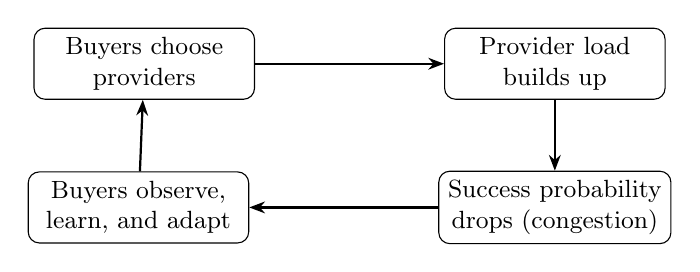
\begin{tikzpicture}[node distance=0.9cm and 2.4cm,
  box/.style={draw, rounded corners, align=center, minimum width=2.8cm, minimum height=0.8cm, font=\small},
  arr/.style={-{Stealth[length=2mm]}, thick}]
  \node[box] (a) {Buyers choose\\providers};
  \node[box, right=of a] (b) {Provider load\\builds up};
  \node[box, below=of b] (c) {Success probability\\drops (congestion)};
  \node[box, left=of c] (d) {Buyers observe,\\learn, and adapt};
  \draw[arr] (a) -- (b); \draw[arr] (b) -- (c); \draw[arr] (c) -- (d); \draw[arr] (d) -- (a);
\end{tikzpicture}
\caption{The feedback loop between learning buyers and congestible providers.}
\label{fig:loop}
\end{figure}

\textbf{Approach and Positioning.} Buyers use a sliding-window contextual Thompson Sampling learner \cite{thompson1933,russo2018} with Bandits-with-Knapsacks (BwK) budget pacing \cite{badanidiyuru2013,agrawal2016}, and observe only a \emph{lagged} public load signal, which is produced by the learners themselves. Contextual BwK guarantees assume exogenous contexts \cite{agrawal2016}; learning in congestion games \cite{rosenthal1973,roughgarden2002,kleinberg2009} and multi-player bandits with collisions \cite{rosenski2016,boursier2019} study interacting learners without a hard budget; budget pacing has been studied in repeated auctions \cite{balseiro2019}, where the pacer is not also learning congestible reliabilities; and non-stationarity is classically handled by sliding windows \cite{garivier2011} (see \cite{slivkins2019,busoniu2008} for background). Our contribution is empirical: we test whether the combination survives policy-induced non-stationarity under strict budgets, and, borrowing the deviation logic of empirical game-theoretic analysis \cite{wellman2006}, whether a self-interested buyer would adopt it. The research gap is:
\begin{quote}\itshape
How does decentralized learning behave when budget constraints, load-dependent congestion and endogenous contextual feedback occur simultaneously, and is the learning rule that helps the market also the one each buyer would choose?
\end{quote}
\textbf{The Precise Computational Question.} \emph{When does budget pacing become valuable under endogenous congestion, and for whom?} Specifically: (1)~does load-aware context help; (2)~does sliding-window forgetting help; (3)~does pacing help; (4)~does the full system's advantage over a vanilla learner grow when contention and tightness rise together; and (5)~does a single buyer gain by switching to PACE when others do not, and lose by switching away when everyone uses it? These are hypotheses H1--H5 in Section~\ref{sec:formulation}.

\section{Preliminaries}
\textbf{Known and unknown.} Globally known are the provider count $N$, the fixed prices $p_i$, the form of the congestion rule and the lagged load $n_i(t-1)$. Because prices are public and increase with quality, buyers can infer the \emph{ordinal} ranking of reliabilities; we build this leak into every learner's prior. Unknown are $(q_i^{\max},c_i,\gamma)$ and the competitors' values and budgets.

\textbf{Definitions.} \emph{Thompson Sampling (TS)} samples a success probability for each option from its Beta posterior and acts greedily on the samples. \emph{Budget pacing} spreads a finite budget over the remaining horizon through a multiplier $\phi_k(t)$ that inflates the perceived price. The \emph{herding index} $\mathrm{HHI}_t=\sum_i\big(n_i(t)/\sum_jn_j(t)\big)^2$ is $1$ if all buyers pick one provider and $1/N$ under an even split. \emph{Common random numbers (CRN)} reuse the same environments and random streams across variants and cells, so comparisons are paired.

\begin{table}[h]
\centering\small
\caption{Environment parameters. Every cell of the $3\times3$ grid reuses the same base draws, rescaled.}
\label{tab:env}
\begin{tabular}{p{2.6cm} p{12.2cm}}
\toprule
\textbf{Parameter} & \textbf{Description / Distribution} \\
\midrule
$N, K, T$ & $5$ providers, $50$ buyers, $T=5{,}000$ rounds. \\
$V_k$ & Private value per success, $V_k\sim\mathrm{Uniform}(4,10)$. \\
$q_i^{\max}, c_i$ & $q_i^{\max}\sim\mathrm{Uniform}(0.5,1)$; base capacity $c_i\sim\mathrm{Uniform}(5,20)$. \\
Prices $p_i$ & Providers sorted by $q_i^{\max}$; prices \$1.00, 1.50, 2.00, 2.50, 3.00, so $\bar p=2$. \\
$\gamma$ & $1$ in the main experiments; $\{0.5,2\}$ in the robustness checks. \\
Tightness $\tau$ & $\tau=T\bar p/\bar B(0)$ with $B_k(0)\sim\mathrm{Uniform}(0.8,1.2)\cdot T\bar p/\tau$: Slack $0.5$, Moderate $1$, Tight $2$. \\
Contention $\rho$ & $\rho=K/\sum_ic_i$, base capacities rescaled per cell: Low $0.5$, Medium $1$, High $2$. \\
\bottomrule
\end{tabular}
\end{table}

\section{Problem Formulation}
\label{sec:formulation}
\textbf{Game.} A repeated stochastic game $\Gamma=\big(K,N,T,\{V_k,B_k(0)\}_{k},\{q_i^{\max},c_i,p_i\}_{i},\gamma\big)$. Providers are indexed in increasing order of $q_i^{\max}$; action $0$ is abstaining, with $p_0=0$ and $q_0\equiv0$. For $k\in[K]$, $t\in[T]$:
\begin{align}
&a_k(t)\in\mathcal{A}_k(t)=\{0\}\cup\{i\in[N]:p_i\le B_k(t)\},\qquad n_i(t)=\textstyle\sum_{k}\mathbf 1\{a_k(t)=i\},\\
&X_k(t)\mid a_k(t)\sim\mathrm{Bernoulli}\big(q_{a_k(t)}(t)\big),\qquad B_k(t+1)=B_k(t)-p_{a_k(t)},\\
&q_i(t)=q_i^{\max}\min\big\{1,(c_i/n_i(t))^{\gamma}\big\}\ \text{ if } n_i(t)>0,\qquad q_i(t)=q_i^{\max}\ \text{ otherwise.}\label{eq:congestion}
\end{align}

\textbf{Information and round protocol.} Buyer $k$ observes $h_k(t)=\big(B_k(t),\,n(t-1),\,(a_k(s),X_k(s))_{s<t}\big)$, never the current load. Each round (1)~every buyer observes $h_k(t)$; (2)~all buyers choose simultaneously; (3)~the joint action fixes $n_i(t)$; (4)~outcomes are drawn from Eq.~\eqref{eq:congestion}; (5)~payments are deducted and each buyer updates only its own posterior. Step~2 makes the problem multi-agent: no buyer can condition on what competitors do in the same round.

\textbf{Buyer problem and system metric.} Each buyer solves
\begin{equation}
\max_{\pi_k}\ \mathbb{E}[U_k],\quad U_k=\sum_{t=1}^{T}\big(V_kX_k(t)-p_{a_k(t)}\big)\quad\text{s.t.}\quad\sum_{t=1}^{T}p_{a_k(t)}\le B_k(0).
\end{equation}
Aggregate surplus $W=\sum_k\mathbb E[U_k]$ is an evaluation metric, not an agent objective.

\textbf{Hypotheses.} Let $W_{s,m}(P,C,S)$ be the surplus of variant $(P,C,S)$ under seed $s$ in cell $m$ when all buyers run it; write Van $=(0,0,0)$, PACE $=(1,1,1)$, and let $G_k(\sigma')=U_k(\mathrm{PACE};\sigma')-U_k(\mathrm{Van};\sigma')$ be buyer $k$'s gain from adopting PACE when the other $K-1$ buyers run $\sigma'$. Using Eqs.~\eqref{eq:anova}--\eqref{eq:envreg}:
\begin{align*}
&\text{H1 (context): } \theta_C^{(m)}>0,\quad \text{H2 (window): } \theta_S^{(m)}>0,\quad \text{H3 (pacing): } \theta_P^{(m)}>0 \quad\text{for at least one cell } m;\\
&\text{H4 (interaction): } \lambda_3>0 \text{ for } \Delta W_{s,m}=W_{s,m}(\mathrm{PACE})-W_{s,m}(\mathrm{Van});\\
&\text{H5 (incentives), per cell: } \bar G^{(m)}(\mathrm{Van})>0 \text{ and } \bar G^{(m)}(\mathrm{PACE})>0.
\end{align*}
H5a (invasion) asks whether a lone PACE buyer in a vanilla market gains; H5b (stability) whether a buyer in an all-PACE market loses by switching back.

\section{Methodology}
\label{sec:method}
\subsection{The PACE learner}
\label{sec:algorithms}
Every learning variant is built on one Beta--Bernoulli TS core with three switches $(P,C,S)\in\{0,1\}^3$, so the factorial comparison isolates the marginal value of each mechanism; vanilla is $(0,0,0)$ and PACE is $(1,1,1)$. Algorithm~\ref{alg:pace} gives one round for one buyer.

\begin{algorithm}[h]
\caption{One round of the TS core for buyer $k$, with switches $P$ (pacing), $C$ (context), $S$ (window)}
\label{alg:pace}
\small
\begin{algorithmic}[1]
\Require posteriors $(\alpha_{i,b},\beta_{i,b})$ initialized to $(p_i,\,4-p_i)$; window $L$; step $\eta$; budget $B_k(t)$; multiplier $\phi_k(t)$
\State Observe the lagged load $n(t-1)$; for every provider set $b_i\gets b(n_i(t-1))$ if $C=1$, else $b_i\gets0$
\If{$S=1$ and an observation $(i',b',x')$ was stored in round $t-L$}
  \State $\alpha_{i',b'}\gets\alpha_{i',b'}-x'$, \ $\beta_{i',b'}\gets\beta_{i',b'}-(1-x')$ \Comment{forget it}
\EndIf
\For{every provider $i$ with $p_i\le B_k(t)$}
  \State $\tilde q_i\gets F^{-1}_{\mathrm{Beta}(\alpha_{i,b_i},\beta_{i,b_i})}(u_{t,k,i})$ \Comment{exact Thompson sample from a pre-drawn uniform}
\EndFor
\State $a\gets\arg\max\big\{0;\ V_k\tilde q_i-p_i(1+\phi_k(t)) : p_i\le B_k(t)\big\}$ \Comment{$\phi_k\equiv0$ if $P=0$; ties to the lower index}
\State Pay $p_a$; all buyers' choices fix $n_a(t)$ and $q_a(t)$; observe $X_k(t)$
\If{$a\ne0$}
  \State $\alpha_{a,b_a}\gets\alpha_{a,b_a}+X_k(t)$, \ $\beta_{a,b_a}\gets\beta_{a,b_a}+1-X_k(t)$; store $(a,b_a,X_k(t))$ \Comment{bucket seen at decision time}
\EndIf
\If{$P=1$} $\phi_k(t+1)\gets\max\big\{0,\ \phi_k(t)+\eta\big(p_a-B_k(t)/(T-t+1)\big)\big\}$ \EndIf
\State $B_k(t+1)\gets B_k(t)-p_a$
\end{algorithmic}
\end{algorithm}

\textbf{Components.} (i)~\emph{Informed prior} (all variants): $\alpha=p_i$, $\beta=4-p_i$, a prior mean $p_i/4\in[0.25,0.75]$ with four pseudo-observations, which encodes the price--quality leak while letting data dominate quickly. (ii)~\emph{Context} ($C=1$): one posterior per provider and load bucket $b(n)=\min(\lfloor n/5\rfloor,9)$; $C=0$ keeps one posterior per provider. (iii)~\emph{Sliding window} ($S=1$): an observation made in round $s$ is subtracted in round $s+L$ (a ring buffer), so a posterior with no recent data reverts exactly to the prior; $S=0$ never forgets. (iv)~\emph{Pacing} ($P=1$): the multiplier $\phi_k$ is a tunable heuristic motivated by the subgradient of the per-round budget constraint. The feasibility filter $\mathcal A_k(t)$ makes every variant budget-safe. In the Slack regime $B_k(t)/(T-t+1)\ge3.2>p_N$ always, so $\phi_k$ never leaves $0$: pacing is exactly inert there, a built-in negative control for H3.

\subsection{Baselines and the LP upper bound}
\textbf{Baselines.} \emph{Vanilla} cumulative TS with the feasibility filter, $(0,0,0)$; \emph{random}, uniform over $\mathcal A_k(t)$ including abstaining; a \emph{centralized greedy} policy with full information, which each round processes budget-feasible buyers in descending order of $V_k$ and assigns each to the provider with the largest marginal immediate expected surplus, or abstains; and an \emph{LP-guided} full-information policy in which buyer $k$ picks provider $i$ with probability $z^\star_{k,i}/T$ from the LP below (abstaining otherwise or if unaffordable).

\textbf{LP upper bound.} The receding-horizon MIP oracle of the first proposal was replaced by a fluid relaxation \cite{badanidiyuru2013}. Let $z_{k,i}$ be the number of rounds in which buyer $k$ uses provider $i$ at full quality:
\begin{equation}
\WLP=\max_{z\ge0}\sum_{k,i}\big(q_i^{\max}V_k-p_i\big)z_{k,i}\quad\text{s.t.}\quad\sum_kz_{k,i}\le c_iT\ \forall i,\quad\sum_iz_{k,i}\le T\ \forall k,\quad\sum_ip_iz_{k,i}\le B_k(0)\ \forall k.
\label{eq:lp}
\end{equation}
It has $KN=250$ variables and $N+2K=105$ constraints and is solved once per (cell, seed) with HiGHS (median @@lp_ms@@~ms).

\begin{proposition}
\label{prop:lp}
Let $\gamma\ge1$ and $\widetilde W=\sum_k\sum_t\big(V_kq_{a_k(t)}(t)-p_{a_k(t)}\big)$, the sum of the expected payoffs of the actions actually taken. For every budget-feasible policy profile, $\widetilde W\le\WLP$ on every sample path, and $W=\mathbb E[\widetilde W]\le\WLP$.
\end{proposition}
\begin{proof}
For a round in which $n\ge1$ buyers choose $i$, let $w=q_i(t)/q_i^{\max}=\min\{1,(c_i/n)^\gamma\}$. Since $\gamma\ge1$, $w\le1$ and $nw\le c_i$. Each such term satisfies $wq_i^{\max}V_k-p_i\le w(q_i^{\max}V_k-p_i)$ because $p_i\ge wp_i$. With $\tilde z_{k,i}=\sum_tw_{i,t}\mathbf 1\{a_k(t)=i\}$, summing gives $\widetilde W\le\sum_{k,i}(q_i^{\max}V_k-p_i)\tilde z_{k,i}$, and $\tilde z$ is feasible for Eq.~\eqref{eq:lp}: $\sum_k\tilde z_{k,i}=\sum_tn_i(t)w_{i,t}\le c_iT$, $\sum_i\tilde z_{k,i}\le T$, and $\sum_ip_i\tilde z_{k,i}\le\sum_tp_{a_k(t)}\le B_k(0)$. Finally, given the history before round $t$ and the round-$t$ actions, $\mathbb E[X_k(t)]=q_{a_k(t)}(t)$, so $\mathbb E[\widetilde W]=W$ by the tower property.
\end{proof}
Realized surplus is not bounded pathwise and can exceed $\WLP$ by Bernoulli noise. The true optimum lies between the better full-information policy and $\WLP$.

\subsection{Experimental design}
\label{sec:design}
\textbf{Grid, seeds and CRN.} A $3\times3$ grid of contention $\rho\in\{0.5,1,2\}$ and tightness $\tau\in\{0.5,1,2\}$. We drew $50$ base environments: seeds 0--9 (validation) were used only for tuning, and every reported result uses the $40$ holdout seeds. Each environment is rescaled across the grid. All remaining randomness comes from two arrays pre-drawn per seed, $u^x_{t,k}$ for outcomes ($X_k(t)=1$ iff $u^x_{t,k}<q$) and $u_{t,k,i}$ for the Thompson samples; neither depends on any policy, so switching one buyer's strategy changes nobody's random draws.

\textbf{Tuning.} PACE was tuned on the validation seeds by grid search, maximizing its mean $W/\WLP$ over the nine cells. The first grid ($\eta\le0.3$, $L\le1{,}600$) peaked at its corner, so before any holdout run it was extended to $\eta\in\{0.003,\dots,10\}$, $L\in\{100,\dots,3{,}200\}$ (keeping $L<T$). The selected $\eta^\star$ = @@eta@@ is interior (score @@tune_score@@\% of $\WLP$, against @@tune_eta3@@\% at $\eta=3$), whereas the score rose monotonically with $L$ in every row, so $L^\star$ = @@L@@ is the longest window that still forgets: a first sign against H2. Both values were frozen and shared by all variants.

\begin{table}[h]
\centering\small
\caption{Studies. ``Self-play'': every buyer runs the same variant.}
\label{tab:studies}
\begin{tabular}{@{}l l p{9.6cm} r@{}}
\toprule
\textbf{Study} & \textbf{Tests} & \textbf{Design} & \textbf{Runs}\\
\midrule
A. Components & H1--H3 & All 8 $(P,C,S)$ configurations, self-play, every cell and holdout seed & 2,880\\
B. Environment & H4 & Vanilla and PACE runs of A, pooled over the nine cells & --\\
C. Incentives & H5 & One deviant (10th/30th/50th/70th/90th percentile of $V_k$) runs PACE among 49 vanilla buyers (invasion) or vanilla among 49 PACE buyers (stability) & 3,600\\
D. Benchmarks & -- & Random, greedy and LP-guided policies; LP bound for every (cell, seed) & 1,080\\
E. Robustness & -- & Five one-at-a-time checks $\times$ two alternatives, vanilla and PACE, cells High/Tight and Low/Slack, 20 seeds & 800\\
F. Shares (ext.) & -- & PACE adopted by 25\%, 50\% or 75\% of buyers, spread evenly over value ranks & 1,080\\
\bottomrule
\end{tabular}
\end{table}

\textbf{Metrics.} The primary metric is surplus as a percentage of $\WLP$ (H1--H4) and the unilateral gain $G_k$ (H5). We estimate expected surplus by $\widetilde W$ of Proposition~\ref{prop:lp}, which replaces each success indicator by its probability given the history and the round's actions; it has the same expectation as realized surplus and makes Proposition~\ref{prop:lp} a check on every run. Diagnostics explain \emph{why} an effect appears and are not tested: load volatility (coefficient of variation of $n_i(t)$), herding (HHI), voluntary abstention, budget exhaustion (share of buyers who can no longer afford the cheapest provider before $T$) and the average price per attempt.

\textbf{Statistical tests.} For H1--H3 we fit, per cell, a factorial ANOVA on seed-level surplus with a seed fixed effect $\delta_s$ (exploiting the CRN pairing) and effect-coded factors $P,C,S\in\{-1,+1\}$:
\begin{equation}
W_{s,m}=\theta_0+\theta_PP+\theta_CC+\theta_SS+\theta_{PC}PC+\theta_{PS}PS+\theta_{CS}CS+\theta_{PCS}PCS+\delta_s+\epsilon_{s,m},
\label{eq:anova}
\end{equation}
so $\theta_F$ is half the average on/off effect of component $F$. Each $\theta_F^{(m)}$ is tested one-sided ($t$-test, 273 residual degrees of freedom), Bonferroni-corrected over the nine cells ($p<0.05/9$). For H4 we regress, with seed fixed effects,
\begin{equation}
\Delta W_{s,m}=\lambda_0+\lambda_1\tilde\rho_m+\lambda_2\tilde\tau_m+\lambda_3\tilde\rho_m\tilde\tau_m+\delta_s+\epsilon_{s,m},\qquad \tilde\rho_m=\log_2\rho_m,\ \tilde\tau_m=\log_2\tau_m,
\label{eq:envreg}
\end{equation}
with intervals from a 10,000-replication bootstrap that resamples whole seeds. For H5, $\bar G^{(m)}$ averages over seeds and the five deviants and is tested one-sided with a seed-level bootstrap, Bonferroni-corrected. Table~\ref{tab:reading} shows how each cell is read.

\begin{table}[h]
\centering\small
\caption{Reading the incentive study in each cell; ``$>0$'' means significantly positive after correction.}
\label{tab:reading}
\begin{tabular}{@{}l p{6.2cm} p{6.2cm}@{}}
\toprule
 & $\bar G^{(m)}(\mathrm{Van})>0$: a lone adopter gains & $\bar G^{(m)}(\mathrm{Van})\le0$: a lone adopter does not gain\\
\midrule
$\Delta W_m>0$ & \emph{Aligned}: the market gain is self-enforcing; H5b tests stability & \emph{Social dilemma}: PACE helps the market, but no buyer adopts it alone\\
$\Delta W_m\le0$ & \emph{Tragedy}: each buyer adopts PACE, and the market loses & \emph{Not worth adopting}\\
\bottomrule
\end{tabular}
\end{table}

\textbf{Implementation checks and reproducibility.} Automated tests confirm that the context is always $b(n_i(t-d))$, never $b(n_i(t))$; no buyer overspends; no run's $\widetilde W$ exceeds $\WLP$; $P=0$ keeps $\phi\equiv0$, $C=0$ uses one posterior and $S=0$ never evicts; the windowed posterior equals the prior plus exactly the last $L$ observations; all variants share the prior; results are identical whether a run is simulated alone or in a batch; and pacing is inert when budgets are Slack. Over all @@lp_check_runs@@ runs with $\gamma=1$, no $\widetilde W$ exceeded $\WLP$; the full-information policies attain it, up to rounding, in @@n_at_bound@@ Low/Slack environments, and realized surplus exceeded it by at most @@lp_excess_real@@\%. The @@n_runs@@ runs took @@cpu_h@@ CPU-hours (about @@wall_min@@ minutes on 15 cores of a laptop); the code, raw run data and scripts that regenerate every number and figure accompany this report.

\section{Results}
\label{sec:results}
\subsection{Overview and benchmarks}
\label{sec:overview}
Table~\ref{tab:bench} puts every policy on the scale of $\WLP$. In every cell the better full-information policy reaches at least @@bestfi_HT@@\% of the bound, so the bound is a meaningful yardstick.

@@bench_table@@

\textbf{High contention defeats every decentralized learner.} In High/Slack and High/Moderate all eight learning variants reach only @@pct_011_HS@@--@@pct_000_HM@@\% of the bound, while greedy reaches @@pct_greedy_HS@@\% and @@pct_greedy_HM@@\%. A buyer's private value of attempting ($V_kq_i-p_i>0$) ignores the success probability it takes from others, so buyers over-enter (vanilla abstains voluntarily in only @@vab_000_HS@@ of buyer-rounds in High/Slack). None of PACE's components addresses this externality.

\textbf{The planned sanity check failed.} Vanilla beats random on average in all nine cells, but seed by seed only in @@vr_HT@@--@@vr_HM@@ of 40 environments in the Tight cells and under High contention. Unpaced TS maximizes per-round surplus and runs out of money halfway (@@exh_000_LT@@ of vanilla buyers are broke before $T$ in Low/Tight, at a median round of @@exhmed_000_LT@@), while random spends more slowly; under High contention, random's one-in-six abstentions relieve congestion. PACE beats random in all 40 seeds in @@n_pr40@@ cells, but only in @@pr_HS@@ and @@pr_HM@@ of 40 in High/Slack and High/Moderate.

\subsection{H1--H3: which components help?}
\begin{figure}[h]
\centering
\includegraphics[width=0.9\linewidth]{figures/fig2_main_effects.pdf}
\caption{Main effects $\theta_F^{(m)}$ of pacing, context and the window per cell, in \% of $\WLP$, with 95\% confidence intervals from Eq.~\eqref{eq:anova}; filled markers are significant after Bonferroni correction. The panels use different horizontal scales.}
\label{fig:effects}
\end{figure}

\textbf{H3 (pacing): supported.} $\theta_P$ is significantly positive in @@nPpos@@ cells, every Moderate and Tight cell except High/Moderate (Figure~\ref{fig:effects}); switching pacing on adds @@th2P_LT@@, @@th2P_MT@@ and @@th2P_HT@@ of $\WLP$ in the three Tight cells, and $\theta_P$ is exactly zero in the Slack column, as the negative control requires. Figure~\ref{fig:diag} shows the mechanism: in the Tight cells @@exh_000_HT@@--@@exh_000_MT@@ of vanilla buyers go broke before $T$, against @@exh_100_HT@@--@@exh_100_LT@@ with pacing alone; paced buyers abstain voluntarily in @@vab_100_LT@@--@@vab_100_HT@@ of rounds and buy cheaper attempts (average price \$@@spa_000_LT@@ $\to$ \$@@spa_100_LT@@ in Low/Tight). In High/Moderate the main effect is zero and pacing alone lowers surplus (@@pct_100_HM@@\% vs.\ @@pct_000_HM@@\% for vanilla): @@exh_000_HM@@ of vanilla buyers go broke there against @@exh_100_HM@@ with pacing, consistent with going broke acting as an \emph{exit} that relieves congestion for the rest.

\begin{figure}[h]
\centering
\includegraphics[width=0.88\linewidth]{figures/fig3_diagnostics.pdf}
\caption{Diagnostics for vanilla, pacing only (P), context only (C) and PACE, means over 40 seeds. Standard errors are at most @@se_hhi@@ (HHI), @@se_vab@@ (abstention) and @@se_exh@@ (share broke); the load CV is inflated for P in Low/Tight because expensive providers are then used only sporadically.}
\label{fig:diag}
\end{figure}

\textbf{H1 (context): not supported.} $\theta_C$ is never significantly positive (largest @@thC_LM@@, $p=@@thCp_LM@@$), and a supplementary test finds it significantly \emph{negative} in @@nCneg@@ of 9 cells, by up to @@thC_HS@@. The harm depends on pacing: the pacing--context interaction is positive and significant in @@pc_sig_cells@@. Without pacing, context changes surplus by @@cP0_LT@@ in Low/Tight, where contextual buyers pay more per attempt (\$@@spa_010_LT@@ vs.\ \$@@spa_000_LT@@) and go broke more often (@@exh_010_LT@@ vs.\ @@exh_000_LT@@); with pacing it changes it by @@cP1_LT@@. Under Medium and High contention context also raises load volatility (High/Slack CV @@cv_000_HS@@ $\to$ @@cv_010_HS@@), consistent with all buyers reacting to the same stale signal, the El Farol pattern \cite{arthur1994}.

\textbf{H2 (window): not supported.} $\theta_S$ is never significantly positive (smallest $p=@@thSp_LS@@$) and is significantly negative in @@nSneg@@ cells (at most @@thS_HS@@). Like context, the window turns slightly positive once pacing is on in Low/Tight and Medium/Tight (@@sP1_LT@@, @@sP1_MT@@, not significant), which is why full PACE beats pacing alone in exactly those two cells; pacing alone matches or beats PACE in the other @@n_p_beats_other@@.

\subsection{H4: does PACE's advantage grow with contention and tightness together?}
\begin{figure}[h]
\centering
\includegraphics[width=0.5\linewidth]{figures/fig4_dW_heatmap.pdf}
\caption{Self-play gain $\Delta W$ of PACE over vanilla, in percentage points of $\WLP$, with 95\% seed-bootstrap intervals.}
\label{fig:heat}
\end{figure}

\textbf{H4: supported.} $\lambda_3$ = @@l3_abs@@ per unit of $\tilde\rho\tilde\tau$ (95\% CI @@l3ci_abs@@, one-sided $p<10^{-4}$), and it stays positive relative to vanilla surplus (@@l3_rel@@, CI @@l3ci_rel@@) and in points of $\WLP$ (@@l3_pct_lp@@, CI @@l3ci_pct_lp@@). PACE's largest gain, @@dwpct_HT@@ (@@dwrel_HT@@ over vanilla), is in High/Tight (Figure~\ref{fig:heat}). Two caveats: in this balanced design $\lambda_3=\tfrac14(\Delta W_{HT}-\Delta W_{HS}-\Delta W_{LT}+\Delta W_{LS})$ depends only on the corner cells, and the pattern is not monotone: $\Delta W$ is negative in every Slack cell, falls with contention in the Moderate column (@@dwpct_LM@@, @@dwpct_MM@@, @@dwpct_HM@@), and is smallest at Medium contention in the Tight column.

\subsection{H5: would a self-interested buyer adopt PACE?}
\begin{figure}[h]
\centering
\includegraphics[width=0.9\linewidth]{figures/fig5_incentives.pdf}
\caption{Left: each cell placed by its self-play gain $\Delta W$ and the invasion gain $\bar G(\mathrm{Van})$ of a lone PACE adopter; quadrants are the categories of Table~\ref{tab:reading} (codes: contention L/M/H, tightness S/M/T). Right: invasion and stability gains with 95\% bootstrap intervals; filled = significantly positive.}
\label{fig:inc}
\end{figure}

@@incentive_table@@

\textbf{H5: supported in five cells, rejected in four} (Table~\ref{tab:inc}, Figure~\ref{fig:inc}). In the five Moderate and Tight cells other than High/Moderate, PACE is \emph{aligned and stable}. Under Tight budgets the invasion gains (@@ginv_LT@@, @@ginv_MT@@, @@ginv_HT@@ per buyer, i.e.\ @@ginvrel_LT@@ to @@ginvrel_HT@@ of the buyer's vanilla payoff) far exceed the stability gains (@@gstab_LT@@, @@gstab_MT@@, @@gstab_HT@@), consistent with the ``late market'' effect: a lone adopter profits most when vanilla buyers go broke around round 2,500 and leave it a half-empty market. Gains rise with the buyer's value (in Low/Tight from @@ginvq10_LT@@ at the 10th to @@ginvq90_LT@@ at the 90th percentile). In the Slack cells PACE is \emph{not worth adopting}: pacing is inert and only the costs of context and forgetting remain. \emph{High/Moderate is a tragedy}: a lone adopter gains @@ginv_HM@@, yet universal adoption lowers surplus by @@dwabs_HM@@ and the all-PACE market is not stable ($\bar G(\mathrm{PACE})$ = @@gstab_HM@@).

\begin{figure}[h]
\centering
\includegraphics[width=0.7\linewidth]{figures/fig6_shares.pdf}
\caption{Extension: mean gain of PACE adopters and of vanilla buyers relative to their own all-vanilla payoff, by adoption share (points at $1/50$ and $49/50$ are the lone deviants of study C). Bands: 95\% intervals over seeds.}
\label{fig:shares}
\end{figure}

\textbf{Population shares.} In Low/Moderate, Low/Tight, Medium/Moderate and Medium/Tight adopters gain more than holdouts at every share, so PACE is dominant (Figure~\ref{fig:shares}). In High/Tight holdouts \emph{gain} as PACE spreads (@@sh_van_098_HT@@ for a lone vanilla buyer in an all-PACE market), so PACE also relieves congestion for others. In High/Moderate the adopters' gain falls from @@sh_pace_002_HM@@ alone to @@sh_pace_100_HM@@ at full adoption and the curves cross between 50\% and 75\% (the intervals overlap there): self-interested buyers settle on a mixed population with @@shW_075_HM@@--@@shW_050_HM@@\% of the bound, below the @@shW_000_HM@@\% of an all-vanilla market.

\subsection{Robustness}
@@robust_table@@
No check changes the sign of $\Delta W$ in either corner cell (Table~\ref{tab:rob}). A staler load signal ($d=2,5$) changes almost nothing, consistent with context carrying little usable information; shorter windows reduce PACE's gain, consistent with H2; the prior strength changes the High/Tight gain by at most about 5\%; and $2\eta^\star$ gives a higher point estimate than the tuned $\eta^\star$ (chosen for the average over cells), with overlapping intervals. In Low/Slack, where pacing is inert, $\Delta W$ is negative in every setting.

\section{Discussion and Limitations}
\textbf{What H4 and H5 say together.} Where budgets bind, PACE is good for the market and for the buyer who adopts it, and in five cells it is stable, so its market gain needs no outside enforcement. Because pacing is the only component with a positive main effect, these gains most likely come from pacing, but the deviation study tested PACE as a bundle, so this attribution is an inference. Part of the private incentive comes at others' expense: under Tight budgets a lone adopter gains two to seven times more than a buyer staying with PACE in an all-PACE market. In High/Moderate this turns into a tragedy; a plausible reading is that going broke is privately costly but relieves congestion, while a paced buyer stays until $T$. Context and the window are also harmful in that cell, so part of PACE's loss there is theirs. The largest inefficiency, however, is not about learning: under High contention every learner reaches only about 40\% of the bound with Slack or Moderate budgets, against more than 90\% for the full-information greedy policy. Each attempt is privately profitable and socially wasteful, and better learning cannot fix a mispriced externality; congestion pricing, admission control or coordination would be needed.

\textbf{Success criteria.} Criterion (i) of the proposal (a significant positive main effect for each component in some cell) holds for pacing and fails for context and forgetting; (ii) $\lambda_3>0$ holds; (iii) PACE passes both incentive tests in all five cells with $\Delta W>0$.

\textbf{Limitations.} $\eta$ and $L$ were tuned for PACE and shared by all variants, and short windows were tested only in two cells. Stability within $\{\mathrm{Van},\mathrm{PACE}\}$ is not a Nash equilibrium of the full game; a buyer might prefer pacing alone, and the single-component deviations that would test this were not run. Eq.~\eqref{eq:envreg} assumes a log-linear effect that the data do not show. $N$, $K$, $T$, the prices and the congestion family are fixed, and the mechanisms in Section~\ref{sec:results} are read from diagnostics, not tested. Bonferroni correction is within each hypothesis, and the tests for negative effects were not in the proposal. All 27 H1--H3 decisions, all 18 H5 decisions and the sign of $\lambda_3$ are unchanged when realized surplus replaces $\widetilde W$.

\section*{Conclusion}
Budget pacing is the mechanism that matters: it raises market surplus in five of the six cells where budgets bind, and PACE, which contains it, is individually rational and stable in those five cells, with an advantage that grows when contention and tightness rise together. Load context and sliding-window forgetting do not help as main effects; they become slightly useful only alongside pacing in two tight-budget cells. Where an adopter's gain comes from outlasting others (high contention, moderate budgets), self-interested adoption is a tragedy of the commons, and the largest losses we measured, from over-entry under high contention, lie beyond what any of these learning mechanisms can fix. As promised in the proposal, components that failed to produce the hypothesized effects are reported as results.

\section{Contribution}
\label{sec:contrib}
Table~\ref{tab:contrib} lists the tasks assigned in the idea review and in our project plan, and whether each was fulfilled.

\begin{table}[H]
\centering\small
\caption{Assigned tasks and their status.}
\label{tab:contrib}
\begin{tabular}{@{}p{8.7cm} l l@{}}
\toprule
\textbf{Task} & \textbf{Assigned to} & \textbf{Fulfilled}\\
\midrule
Problem formulation, model, learning and pacing rules (idea review) & Nayan Daryani & Yes\\
Literature review, hypotheses, experimental and statistical design (idea review) & Pradeep Sain & Yes\\
Simulator (environment, learners, baselines, runner) and automated checks & Nayan (lead) & Yes\\
Tuning of $\eta$ and $L$ on validation seeds & Pradeep (lead) & Yes (grid extended once)\\
Pilot of the deviation study (about 5 seeds) & Pradeep & No (not needed: intervals were narrow)\\
Main runs: factorial, deviation and benchmarks & Both & Yes\\
Analysis and figures (ANOVA, bootstrap regression, incentive study) & Pradeep (lead) & Yes\\
Robustness checks in the two corner cells & Nayan & Yes\\
Optional: population shares; single-component deviations & Both & Yes; No\\
Final report & Both & Yes\\
\bottomrule
\end{tabular}
\end{table}

\textbf{Use of AI tools.} AI tools were used for limited
editorial assistance, including formatting the report and
reviewing the cited literature references for consistency
and completeness. The research, implementation, experiments,
analysis and conclusions were carried out by the authors.
We take responsibility for the content.

\begin{thebibliography}{99}
\small\setlength{\itemsep}{1pt}\setlength{\parskip}{0pt}
\bibitem{thompson1933} Thompson, W. R. (1933). On the likelihood that one unknown probability exceeds another in view of the evidence of two samples. \textit{Biometrika}, 25(3/4), 285--294.
\bibitem{russo2018} Russo, D. J., Van Roy, B., Kazerouni, A., Osband, I., \& Wen, Z. (2018). A tutorial on Thompson sampling. \textit{Foundations and Trends in Machine Learning}, 11(1), 1--96.
\bibitem{rosenthal1973} Rosenthal, R. W. (1973). A class of games possessing pure-strategy Nash equilibria. \textit{International Journal of Game Theory}, 2(1), 65--67.
\bibitem{roughgarden2002} Roughgarden, T., \& Tardos, \'E. (2002). How bad is selfish routing? \textit{Journal of the ACM}, 49(2), 236--259.
\bibitem{badanidiyuru2013} Badanidiyuru, A., Kleinberg, R., \& Slivkins, A. (2013). Bandits with knapsacks. In \textit{Proceedings of the 54th IEEE Symposium on Foundations of Computer Science (FOCS)}.
\bibitem{agrawal2016} Agrawal, S., Devanur, N. R., \& Li, L. (2016). An efficient algorithm for contextual bandits with knapsacks, and an extension to concave objectives. In \textit{Proceedings of the 29th Conference on Learning Theory (COLT)}.
\bibitem{kleinberg2009} Kleinberg, R., Piliouras, G., \& Tardos, \'E. (2009). Multiplicative updates outperform generic no-regret learning in congestion games. In \textit{Proceedings of the 41st ACM Symposium on Theory of Computing (STOC)}.
\bibitem{rosenski2016} Rosenski, J., Shamir, O., \& Szlak, L. (2016). Multi-player bandits -- a musical chairs approach. In \textit{Proceedings of the 33rd International Conference on Machine Learning (ICML)}.
\bibitem{boursier2019} Boursier, E., \& Perchet, V. (2019). SIC-MMAB: Synchronisation involves communication in multiplayer multi-armed bandits. In \textit{Advances in Neural Information Processing Systems (NeurIPS)}.
\bibitem{balseiro2019} Balseiro, S. R., \& Gur, Y. (2019). Learning in repeated auctions with budgets: Regret minimization and equilibrium. \textit{Management Science}, 65(9), 3952--3968.
\bibitem{garivier2011} Garivier, A., \& Moulines, E. (2011). On upper-confidence bound policies for switching bandit problems. In \textit{Algorithmic Learning Theory (ALT)}, LNCS 6925, 174--188.
\bibitem{wellman2006} Wellman, M. P. (2006). Methods for empirical game-theoretic analysis. In \textit{Proceedings of the 21st AAAI Conference on Artificial Intelligence}, 1552--1555.
\bibitem{slivkins2019} Slivkins, A. (2019). Introduction to multi-armed bandits. \textit{Foundations and Trends in Machine Learning}, 12(1--2), 1--286.
\bibitem{busoniu2008} Bu\c{s}oniu, L., Babu\v{s}ka, R., \& De Schutter, B. (2008). A comprehensive survey of multiagent reinforcement learning. \textit{IEEE Transactions on Systems, Man, and Cybernetics, Part C}, 38(2), 156--172.
\bibitem{arthur1994} Arthur, W. B. (1994). Inductive reasoning and bounded rationality. \textit{American Economic Review}, 84(2), 406--411.
\end{thebibliography}

\end{document}
